% updated April 2002 by Antje Endemann
% Based on CVPR 07 and LNCS, with modifications by DAF, AZ and elle, 2008 and AA, 2010, and CC, 2011; TT, 2014; AAS, 2016; AAS, 2020

% \documentclass[runningheads]{llncs}
% \usepackage{graphicx}
% \usepackage{comment}
% \usepackage{amsmath,amssymb,amsfonts,bm} % define this before the line numbering.
% \usepackage{color}
% \usepackage{tabularx}
% \usepackage{appendix}

% % our packages
% \usepackage{import}
% % \usepackage{subcaption}
% \usepackage[caption=false]{subfig}
% \usepackage{mathtools}
% \usepackage{booktabs}

% INITIAL SUBMISSION - The following two lines are NOT commented
% CAMERA READY - Comment OUT the following two lines
% \usepackage{ruler}
% \usepackage[width=122mm,left=12mm,paperwidth=146mm,height=193mm,top=12mm,paperheight=217mm]{geometry}

% Macros
% \def\ci{\perp\!\!\!\perp}
% \newcommand*\diff{\mathop{}\!\mathrm{d}}
% \def\httilde{\mbox{\tt\raisebox{-.5ex}{\symbol{126}}}}


% \begin{document}
% \renewcommand\thelinenumber{\color[rgb]{0.2,0.5,0.8}\normalfont\sffamily\scriptsize\arabic{linenumber}\color[rgb]{0,0,0}}
% \renewcommand\makeLineNumber {\hss\thelinenumber\ \hspace{6mm} \rlap{\hskip\textwidth\ \hspace{6.5mm}\thelinenumber}}
% \linenumbers
% \pagestyle{headings}
% \mainmatter
% \def\ECCVSubNumber{5488}  % Insert your submission number here

% \title{Null-sampling for Interpretable and \\Fair Representations -- Appendix} % Replace with your title

% % INITIAL SUBMISSION 
% \begin{comment}
% \titlerunning{ECCV-20 submission ID \ECCVSubNumber} 
% \authorrunning{ECCV-20 submission ID \ECCVSubNumber} 
% \author{Anonymous ECCV submission}
% \institute{Paper ID \ECCVSubNumber}
% \end{comment}
% %******************

% % CAMERA READY SUBMISSION
% %\begin{comment}
% \titlerunning{Appendix}
% % If the paper title is too long for the running head, you can set
% % an abbreviated paper title here
% %
% \author{Thomas Kehrenberg \and
% Myles Bartlett \and
% Oliver Thomas \and \\
% Novi Quadrianto}
% %
% \authorrunning{T. Kehrenberg et al.}
% % First names are abbreviated in the running head.
% % If there are more than two authors, 'et al.' is used.
% %
% \institute{Predictive Analytics Lab (PAL), University of Sussex, Brighton, UK
% \email{\{t.kehrenberg,m.bartlett,ot44,n.quadrianto\}@sussex.ac.uk}}
% %\end{comment}
% %******************

% \title{Appendix}
% \author{}
% \institute{}
% \maketitle
% \thispagestyle{headings}

\section{Appendix}\label{sec:nifr-appendix}

% \begin{appendix}

\subsection{Model Architectures}%
\label{sec:architectures}
\noindent For both cMNIST and CelebA we parameterise the coupling layers with the same convolutional architecture as in \citet{KinDha18}, consisting of $3$ convolutional layers each with $512$ filters of, in order, sizes $3\times3$, $1\times1$, and $3\times3$.
Following \citet{ardizzone2019guided}, we Xavier initialise all but the last convolutional layer of the $s$ and $t$ sub-networks which itself is zero-initialised so that the coupling layers begin by performing an identity transform. We used a Glow-like architecture \citep{KinDha18} (affine coupling layers together with checkerboard reshaping and invertible $1\times1$ convolutions) for the convolutional INNs. Table \ref{tab:inn_architectures} summarises the INN architectures used for each dataset.

For the image datasets each level of the cVAE encoder consists of two gated convolutional layers \citep{van2016conditional} with ReLU activation. 
At each subsequent level, the number of filters is doubled, starting with an initial value 32 and 64 in the case of CelebA and cMNIST respectively. 
In the case of the Adult dataset, we use an encoder with one fully-connected hidden layer of width $35$, followed by SeLU activation \citep{klambauer2017self}. 
For both cMNIST and CelebA, we downsample to a feature map with spatial dimensions $8\times8$, but with $3$ and $16$ channels respectively. 
For the Adult dataset, the encoding is a vector of size $35$. 
The output layer specifies both the parameters (mean and variance) of the representation's distribution. 
In all cases the KL-divergence is computed with respect to a standard isotropic Gaussian prior. 
Details of the encoder architectures can be found in table \ref{tab:vae_architectures}. The loss pre-factors were sampled from a logarithmic scale; without proper balancing the networks can exhibit instability, especially during the early stages of training.

\begin{table}[tp]
\caption{INN architecture used for each dataset.}
\label{tab:inn_architectures}
\centering
\begin{tabular}{lllll}
\toprule
Dataset & Levels & Level depth & Coupl. chan. & Input to discr. \\ \midrule
UCI Adult                   & 1      & 1     & 35       & Null-samples       \\
cMNIST                      & 3      & 16     & 512      & Encodings               \\
CelebA                      & 3      & 32     & 512      & Encodings        \\ \bottomrule
\end{tabular}
\end{table}

\begin{table}[tp]
\caption{cVAE encoder architecture used for each dataset. The decoder architecture in each case mirrors that of its encoder counterpart through use of transposed convolutions. For the adult dataset we apply $\ell_2$ and cross-entropy losses to the reconstructions of the continuous features and discrete features, respectively.}
\label{tab:vae_architectures}
\centering
\begin{tabular}{lllll}
\toprule
Dataset   & Initial channels & Levels & $\beta$ & Recon. loss \\
\midrule
UCI Adult & 35               & --     & 0       & $\ell_2$ + CE\\
cMNIST    & 32               & 4      & 0.01    & $\ell_2$ \\
CelebA    & 32               & 5      & 1       & $\ell_1$ \\ 
\bottomrule
\end{tabular}
\end{table}

\subsection{Additional results}\label{sec:additional-results}
\paragraph{Detailed results for UCI Adult dataset.}
This census data is commonly used to evaluate models focused on algorithmic fairness.
Following convention, we designate ``gender'' as the $s$ and whether an individual's salary is \$50,000 or greater as $y$.
We show the performance of our approach in comparison to baseline approaches in fig.~\ref{fig:big-adult-chart}.
We evaluate the performance of all models for mixing factors ($\eta$) of value $\{0, 0.1, ..., 1\}$. 
Results shown in fig.~\ref{fig:big-adult-chart} show that whilst our model fails to surpass the baseline models in terms of accuracy for the balanced case (and those close to it), we match or exceed the baseline as $\eta $ moves the dataset to a more imbalanced setting. In terms of fairness metrics,  our approach generally outperforms the baseline models regardless of $\eta$.

\begin{figure}[htb]
  \centering
  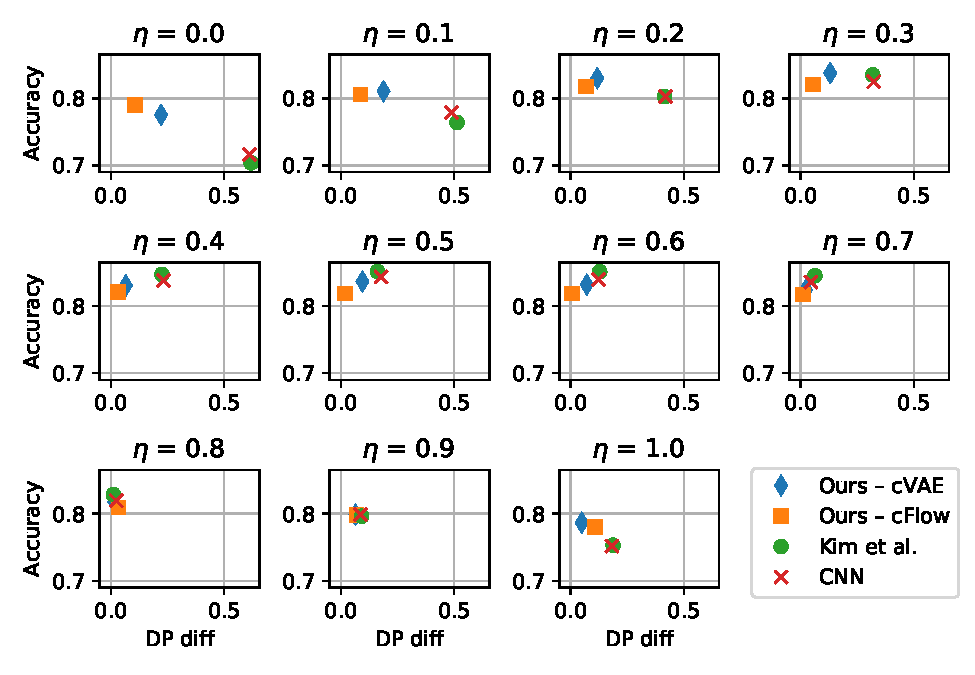
\includegraphics[width=0.85\textwidth]{paper2/Figures/nosinn_adult_multiplot_all_landscape_diff.pdf}
  \caption{
      Results for the \textsc{Adult} dataset.
      The $x$-axis corresponds to the difference in positive rates.
      An ideal result would occupy the \textsc{top-left}.
  }%
  \label{fig:big-adult-chart}
\end{figure}
\begin{figure}[htb]
    \centering
    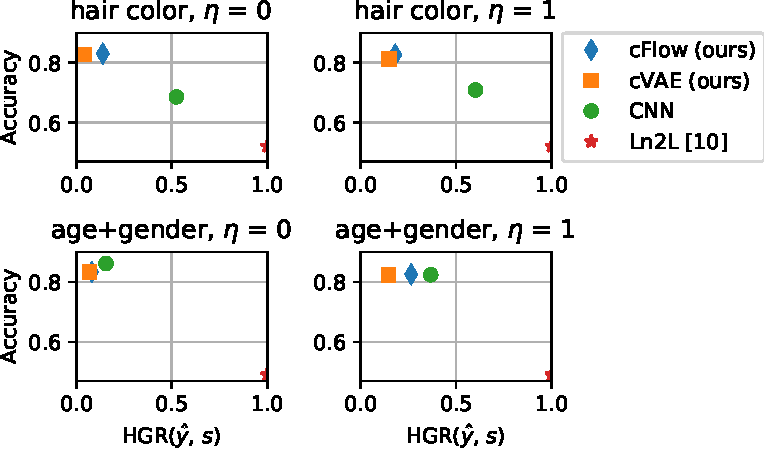
\includegraphics[width=0.7\textwidth]{paper2/Figures/celeba_multi_s.pdf}
    \caption{
        For \emph{hair colour}, $s$ takes on the values Blond, Brown and Black.
        For \emph{age+gender}, $s$ takes on the values Young/Female, Young/Male, Old/Female and Old/Male.
    }%
    \label{fig:multi-s}
\end{figure}

\paragraph{Multinomial sensitive attributes.}
In addition to binary sensitive attribute $s$,
we also investigate multinomial $s$ in the CelebA dataset.
First, we do experiments with hair colour, where $s$ has three possible values:
blond hair, brown hair and black hair.
The other experiment is with a combination of age and gender,
where $s$ has four possible values, each of which is a combination of a gender and an age:
Young/Female, Young/Male, Old/Female and Old/Male.
To evaluate the fairness for multinomial $s$, we use the Hirschfeld-Gebelein-R\'enyi Maximum Correlation Coefficient (HGR) \citep{mary2019fairness} that is defined on the domain $[0, 1]$ and gives $\text{HGR}(Y,S)=0$ iff $Y \perp S$
and 1 if there is a deterministic function to map between them.
Results can be found in figure~\ref{fig:multi-s}.\\

\begin{table}[tp]
\caption{Results on the CelebA dataset with different sizes of $z_b$.}
    \label{tab:zs-ablation}
    \centering
\begin{tabular}{l@{\extracolsep{1cm}}lrr}
\toprule
 $|z_b|$ & $|z_b|/|z|$ &  Accuracy &   DP diff \\
\midrule
          1 &             0.0082\% &  0.60 &  0.63 \\
          3 &             0.0245\% &  0.60 &  0.63 \\
          5 &             0.0410\% &  0.84 &  0.12 \\
         10 &             0.0820\% &  0.84 &  0.12 \\
         30 &             0.2442\% &  0.74 &  0.23 \\
         50 &             0.4070\% &  0.68 &  0.27 \\
\bottomrule
\end{tabular}
\end{table}
\noindent\textsc{Investigation into the size of $z_b$.}
\;\; In the cFlow model, the size of $z_b$ is an important hyperparameter which can affect the result significantly.
Here we investigate the sensitivity of the model to the choice of $z_b$ size.
Table~\ref{tab:zs-ablation} shows accuracy and fairness (as measured by \emph{DP diff}) for different sizes of $z_b$.
The results show that both too large and too small $z_b$ is detrimental.
However, they also show that the model is not overly sensitive to this parameter:
both sizes 5 and 10 achieve nearly identical results.

\begin{table}[tbp]
    \caption{
        Additional fairness metrics for the experiments on the CelebA dataset (fig.~\ref{fig:celeba-multiplot} from the main text).
        \emph{TPR diff.}\ refers to the difference in true positive rate.
        \emph{TNR diff.}\ refers to the difference in true negative rate.
        \textsc{Left:} $\eta = 0$. \textsc{Right:} $\eta=1$.
    }
    \label{tab:my_label}
    \resizebox{.49\textwidth}{!}{
    \begin{tabular}{lrrrr}
\toprule
     Method &  Accuracy &  DP diff &  TPR diff &  TNR diff \\
\midrule
      cFlow &      0.83 &     0.10 &      0.15 &      0.25 \\
       cVAE &      0.82 &     0.05 &      0.09 &      0.18 \\
        CNN &      0.61 &     0.63 &      0.70 &      0.64 \\
 Ln2L &      0.52 &     0.00 &      0.00 &      0.00 \\
\bottomrule
\end{tabular}}
\hfill
\resizebox{.49\textwidth}{!}{
\begin{tabular}{lrrrr}
\toprule
     Method &  Accuracy &  DP diff &  TPR diff &  TNR diff \\
\midrule
      cFlow &      0.82 &     0.33 &      0.28 &      0.21 \\
       cVAE &      0.81 &     0.16 &      0.10 &      0.05 \\
        CNN &      0.67 &     0.75 &      0.66 &      0.76 \\
Ln2L &      0.51 &     0.08 &      0.06 &      0.09 \\
\bottomrule
\end{tabular}}
\end{table}
\paragraph{Additional fairness metrics.}
In addition to \emph{DP diff}, we report here the result from other fairness measures.
These results are from the same setup as those reported in the main paper.
We report the difference in true positive rates (TPR) between the two groups (male and female), which corresponds to a measure of Equality of Opportunity,
and the difference in true negative rates (TNR) between the two groups.

\subsection{Optimisation Details}\label{sec:optimisation-details}
\noindent All our models were trained using the RAdam optimiser \citep{liu2019variance} with learning rates $3\times10^{-4}$ and $1\times10^{-3}$ for the encoder/discriminator pair and classifier respectively. A batch size of 128 was used for all experiments.

We now detail the optimisation settings, including the choice of adversary, specific to each dataset. Details of the cVAE and cFlow architectures can be found in table \ref{tab:vae_architectures} and table \ref{tab:inn_architectures}, respectively.

\paragraph{UCI Adult.} 
For this dataset our experiment benefited from using null-samples as inputs to the adversary of the cFlow model. Unlike for the image datasets, we found a single adversary to be sufficient. This was realised as a multi-layer perceptron (MLP) with one hidden layer, 256 units wide. The INN performs a bijection of the form $f: \mathbb{R}^n \rightarrow \mathbb{R}^n$. However, the adult dataset is composed of mostly discrete (binary/categorical) features. To achieve good performance, we found it necessary to first pre-process the inputs with a pretrained autoencoder, using its encodings as the input to the cFlow model, as well as to the adversary. The learned representations were evaluated with a logistic regression model from scikit-learn \citep{scikit-learn}, using the standard settings. All baseline models were trained for 200 epochs.
The Ln2L \citep{kim2019learning} and MLP baselines share the architecture of the cVAE's encoder, only with a classification layer affixed.

\paragraph{Coloured MNIST.}
Each level of the architecture used for the downstream classifier and na\"ive baseline alike consists of two convolutional layers, each with kernel size 3 and followed by Batch Norm \citep{ioffe2015batch} and ReLU activation. For the Ln2L baseline, we use an a setup identical to that described in \citet{kim2019learning}. Each level has twice the number of filters in its convolutional layer and half the spatial input dimensions as the last. The original input is downsampled to the point of the output being reduced to a vector, to which a fully-connected classification layer is applied.

To allow for an additional level in the INN (the downsampling operations requiring the number of spatial dimensions to be even), the data was zero-padded to a size of $32\times32$. The cVAE and cFlow models were trained for 50 and 200 epochs respectively, using $\ell_2$ reconstruction loss for the former. The downstream classifier and all baselines were trained for 40 epochs. For both of our models, an ensemble of 5 adversaries was applied to the encodings, with each member taking the form of a fully-connected ResNet, 2 blocks in depth, with SeLU activation \citep{klambauer2017self}. The adversaries were reinitialised independently with probability $0.2$ at the end of each epoch. While the adversaries could equally well take  null-samples as input, as done for the Adult dataset, doing so requires the performing of both forward and inverse passes each iteration, which, for the convolutional INNs of the depths we require for the image datasets, introduces a large computational overhead, while also showing to be the less stable of the two approaches in our preliminary experiments.

\paragraph{CelebA.} 
The downstream classifier and na\"ive baseline take the same form as described above for cMNIST, but with an additional level with 32 filters in each of its convolutions at the top of the network. For this dataset we adapt the Ln2L model by simply considering it as an augmentation the na\"ive baseline's objective function, with the entropy loss applied to the output of the final convolutional layer. These models were again trained for 40 epochs, which we found to be sufficient for convergence for the tasks in question. The cVAE and cFlow models were respectively trained for 100 epochs and 30 epochs, using $\ell_1$ reconstruction loss for the former. Compared with cMNIST, the size of the adversarial ensemble was increased to 10, the reinitialisation probability to 0.33, but no changes were made to the architectures of its members.

\paragraph{The Pitfalls of Adversarial Training.}
Adversarial learning has become one of the go-to methods for enforcing invariance in fair representation learning \citep{ganin2016domain} with MMD \citep{louizos2016variational} and HSIC \citep{QuaShaTho19}, being popular non-parametric alternatives.
\citet{ganin2016domain} proposed adversarial learning for domain adaptation problems, with \citet{edwards2016censoring} soon after making this and learning a representation promoting demographic parity.
The adversarial approach carries the benefits of being both efficient and scalable to multi-class categorical variables, which many sensitive attributes are in practice, whereas the non-parametric methods only permit pair-wise comparison.

However, when realised as a neural network, the adversary is both sensitive to the values of the inputs as well as their ordering (though exchangeable architectures, such as \citet{zaheer2017deep} do exist, but which sacrifice expressiveness).
Thus, it can happen that the representation learner optimises for the surrogate objective of eluding the adversary rather than the real objective of expelling $s$-related information.
Moreover, the non-stationarity of the dynamics can lead to cyclic-equilibria, irrespective of the capacity of the adversary.

When working with a partitioned latent space, this behaviour can be averted by instead encouraging $z_b$ to be predictive of $s$, acting as a kind of information ``sink``, as in \citet{JacSmeOya18}.
However, this does not have the guarantee of making $z_u$ invariant to $s$ - there are often many indicators for $s$, not all of which are needed to predict the label perfectly.
Training the network to convergence before taking each gradient step with the representation learner is one way one to attempt to tame the unstable minimax dynamics \citep{feng2019learning}.
However, this does not prevent the emergence of the aforementioned cyclicity.

We try to mitigate the aforementioned degeneracies by maintaining a diverse set of adversaries, as has shown to be effective for GAN training \citep{durugkar2016generative}, and by decorrelating the individual trajectories by intermittently re-initialising them with some small probability following each iteration.

\paragraph{Tuning the Partition Sizes.}
There are several ways of ensuring that the size of $z_b$ is sufficient to capture all s dependencies, but minimal enough that information unrelated to s is maximally preserved
We adopt the straightforward search strategy of, starting from some initial guess, calibrating the value according to accuracy attained by a classifier trained to predict $s$ from $z_b$ on a held-out subset of the representative set, which is measured whenever the adversarial loss plateaus. If the accuracy is above chance level then that suggests the size of the $z_b$ partition, $|z_b|$, needs to be increased to accommodate more information about $s$. If the accuracy is found to be at chance level then are two possibilities: 1) $|z_b|$ is already optimal; 2) $|z_b|$ is large enough that it fully contains both information $s$ as well as that of a portion of $y$. If the former is true, then perturbations around the current value allow us to confirm this; if the latter is true then decreasing the value was indeed the correct decision.

\subsection{Synthesising Coloured MNIST}\label{sec:color-details}
\noindent We use a colourised version of MNIST as a controlled setting investigate learning from biased data in the image domain. In the biased training set, each digit is assigned a unique mean RGB value parameterising the multivariate Gaussian from which its colour is drawn. These values were chosen to be maximally dispersed across the 8-bit colour spectrum and are listed in table \ref{tab:cmnist_rgb_values}. By adjusting the standard deviation, $\sigma$, of the Gaussians, we adjust the degree of bias in the dataset. When $\sigma=0$, there is a perfect and noiseless correspondence between colour and digit class which a classifier can exploit. The classifier can favour the learning of the low-level spurious feature over those higher level features constituent of the digit's class. As the standard deviation increases, the sampled RGB values are permitted to drift further from the mean, leading to overlap between the samples of the colour distributions and reducing their reliability as indicators of the digit class. In the test and representative sets alike, however, the colour of each sample is sampled from one of the 10 distributions randomly, such that colour can no longer be leveraged as a shortcut to predicting the digit's class.

\subsection{Stabilising the Coupling layers}\label{sec:those-darn-coupling-layers}
\noindent Heuristically, we found that  applying an additional nonlinear function to the scale coefficient of the form
\begin{align}
  s = \sigma (f(u)) + 0.5
  \label{eq:heuristic-1}
\end{align}
greatly improved the stability of the affine coupling layers. Here, $\sigma$ is the logistic function, which we shift to be centred on 1 so that zero-initialising $f$ results in the coupling layers initially performing an identity-mapping.

\begin{table}[tp]
\caption{Mean RGB values (in practice normalised to $[0, 1]$) parameterising the Multivariate Gaussian distributions from which each digit's colour is sampled in the biased (training) dataset. In the representative and test sets,  the colour of each digit is sampled from one of the specified Gaussian distributions at random.}
\label{tab:cmnist_rgb_values}
\centering
\begin{tabular}{l@{\extracolsep{1cm}}lll}
\toprule
Digit & Colour Name & Mean RGB      \\ \midrule
0     & Cyan        & (0, 255, 255) \\
1     & Blue        & (0, 0, 255)   \\
2     & Magenta     & (255, 0, 255) \\
3     & Green       & (0, 128, 0)   \\
4     & Lime        & (0, 255, 0)   \\
5     & Maroon      & (128, 0, 0)   \\
6     & Navy        & (0, 0, 128)   \\
7     & Purple      & (128, 0, 128) \\
8     & Red         & (255, 0, 0)   \\
9     & Yellow      & (255, 255, 0) \\ \bottomrule
\end{tabular}
\end{table}

\subsection{Qualitative Results for CelebA}\label{sec:qual-results-celeba}
\noindent Learning a representation alongside its inverse mapping, be it approximate or exact, enables us to probe the behaviour of the model that produced it,
and any biases it may have implicitly captured due to entanglement between the sensitive attribute and other attributes present in the data.
We highlight a few examples of such biases manifesting in the cFlow model's CelebA null-samples in fig.~\ref{fig:celeba_cflow_suppmat}. In these cases, makeup and hair style have been inadvertently modified during the null-sampling due to the tight correlation between these two attributes and the sensitive attribute, gender, to which we had aimed to make our representations invariant. Additionally, in all highlighted images, the skin tone has changed: from male to gender-neutral, the skin becomes lighter and from female to gender-neutral, the skin becomes darker; in the change from male to gender-neutral, glasses are also often removed.
As the model cannot know that the label is meant to only refer to gender, and not to these other (correlated) attributes,
the links cannot be disentangled by the model.
However, the advantage of our method is that we can at least identify such biases due to the interpretability that comes with the representations being in the data domain.

% \newpage
\begin{figure*}[tb]
  \centering
  \subfloat[Original images.]{%
      \scalebox{0.3}{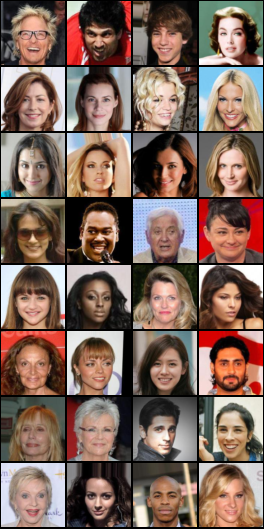
\includegraphics[width=\textwidth]{paper2/Images/celeba/vae_x_original.png}}%
      \label{fig:cvae_celeba_original_x}
  }
  \hfill
  \subfloat[$\bm{x}_u$ null-samples generated by the cVAE model.]{%
      \scalebox{0.3}{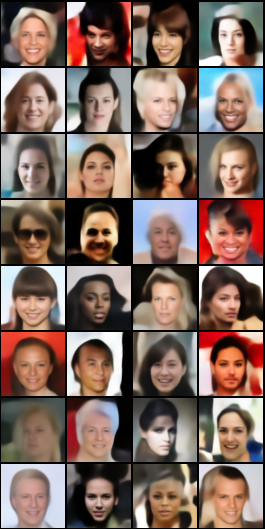
\includegraphics[width=\textwidth]{paper2/Images/celeba/vae_recon_y.png}}%
      \label{fig:cvae_celeba_recon_y}
  }
  \hfill
  \subfloat[$\bm{x}_b$ null-samples generated by the cVAE model.]{%
      \scalebox{0.3}{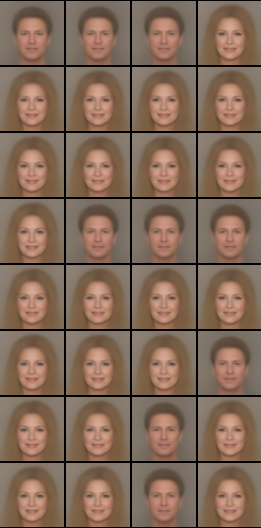
\includegraphics[width=\textwidth]{paper2/Images/celeba/vae_recon_s.png}}%
      \label{fig:cvae_celeba_recon_s}
  }
  \caption{
    CelebA null-samples learned by our cVAE model, with gender as the sensitive attribute.
    (a) The original, untransformed samples from the CelebA dataset
    (b) Reconstructions using only information unrelated to $s$.
    (c) Reconstruction using only information related to $\neg s$.
    The model learns to disentangle gender from the non-gender related information. Compared with the cFlow model, there is a severe degradation in reconstruction quality due to the model trying to simultaneously satisfy conflicting objectives.
    % Attributes such as \emph{makeup} and \emph{hair length} are also often modified in the process due to inherent correlations between them and the sensitive attribute, which the intepretability of our representations allows us to easily identify.
  }\label{fig:celeba_vae}
\end{figure*}

\begin{figure*}[tb]
  \centering
  \subfloat[Original images.]{%
      \scalebox{0.3}{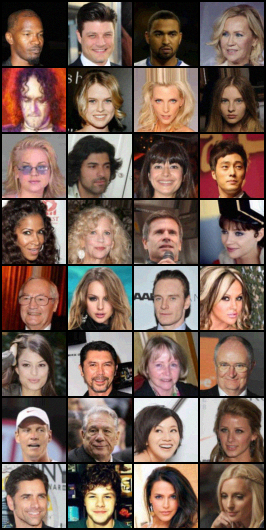
\includegraphics[width=\textwidth]{paper2/Images/celeba/cflow_original_x_suppmat.png}}%
      \label{fig:cflow_celeba_original_x_suppmat}
  }
  \hfill
  \subfloat[$\bm{x}_u$ null-samples generated by the cFlow model.]{%
      \scalebox{0.3}{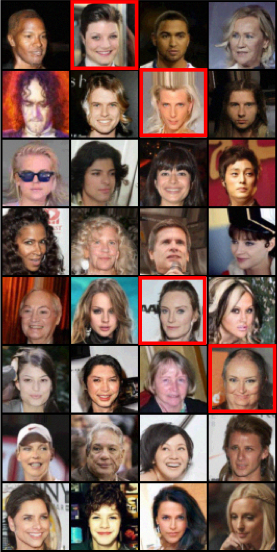
\includegraphics[width=\textwidth]{paper2/Images/celeba/cflow_xd_suppmat.png}}%
      \label{fig:cflow_celeba_recon_y_suppmt}
  }
  \hfill
  \subfloat[$\mathbf{x}_b$ null-samples generated by the cFlow model.]{%
      \scalebox{0.3}{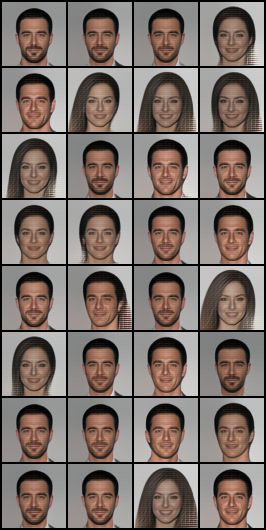
\includegraphics[width=\textwidth]{paper2/Images/celeba/cflow_xb_suppmat.png}}%
      \label{fig:cflow_celeba_recon_s_suppmat}
  }
  \caption{
    CelebA null-samples learned by our cFlow model, with gender as the sensitive attribute.
    (a) The original, untransformed samples from the CelebA dataset
    (b) Reconstructions using only information unrelated to $s$.
    (c) Reconstruction using only information related to $\neg s$.
    The model learns to disentangle gender from the non-gender related information.
    Attributes such as \emph{makeup} and \emph{hair length} are also often modified in the process (prime examples framed with red) due to inherent correlations between them and the sensitive attribute, which the interpretability of our representations allows us to easily identify.
  }\label{fig:celeba_cflow_suppmat}
\end{figure*}



\subsection{Transfer Learning}\label{sec:transfer-learning}
For our method, we require a representative set which follows the same distribution as that observed during deployment.
Such a representative set might not always be available.
In such a scenario, we can resort to using a set that is merely \emph{similar} to that in the deployment setting and leverage transfer learning.

%We argue that the inherent properties of INNs make them especially suitable for transfer learning.
One of the advantages of using an invertible architecture over conventional, \emph{surjective} ones that we stressed in the main text is its \emph{losslessness}. Since the transformations are necessarily bijective, the information contained in the input can never be destroyed, only redistributed. This makes such models particularly well-suited, in our minds, for transferring learned invariances:
even if the input is unfamiliar, no information should be lost when trying to transform it.
This works as long as only the information about $s$ ends up in the $z_b$ partition.
If $s$ takes a form similar to that which we pre-trained on, and can thus be correctly partitioned in the latent space, by complement we have the information about $\neg s$ stored in the $z_u$ partition, without presupposing similarity to the $\neg s$ observed during pre-training.

\paragraph{Transferring from mixed-NIST to MNIST.}
We test our hypothesis by comparing the performance of the cFlow and cVAE models pre-trained on a mixture of datasets belonging to the NIST family, colourised in the same way as cMNIST, while the downstream train and test sets remain the same as in the original cMNIST experiments. Specifically, we create this representative set by sampling 24,000 images (to match the cardinality of the original representative set) from EMNIST (letters only)~\citep{cohen2017emnist}, Fashion\-MNIST~\citep{xiao2017fashion} and KMNIST~\citep{clanuwat2018deep}, in equal proportion. We use the same architectures for the cVAE and cFlow models as we did in the non-transfer learning setting. In terms of hyperparameters, the only change made was to the KL-divergence's pre-factor, finding it necessary to increase it to $1$ to guarantee stability.

The results for the range of $\sigma$ values are shown in fig.~\ref{fig:cmnist-transfer}. Unsurprisingly, the performance of both models suffers when the representative and test sets do not completely correspond. However, the cFlow model consistently outperforms the cVAE model, with the gap increasing as the bias decreases.
Although some colour information is retained in the cFlow null-samples, symptomatic of an imperfect transfer, semantic information is almost entirely retained as well.
Conversely, the cVAE is very much flawed in this respect; as can be seen in the bottom row of fig.~\ref{fig:cmnist-transfer}, for some samples, semantic information is degraded to the point of the digit's identity being altered. As a result of this semantic degradation, the performance of the downstream classifier is curtailed by the noisiness of the digit's identity and is relatively unchanging across $\sigma$-values, in contrast to the monotonic improvement of that achieved on the cFlow null-samples.
% \begin{figure}
%   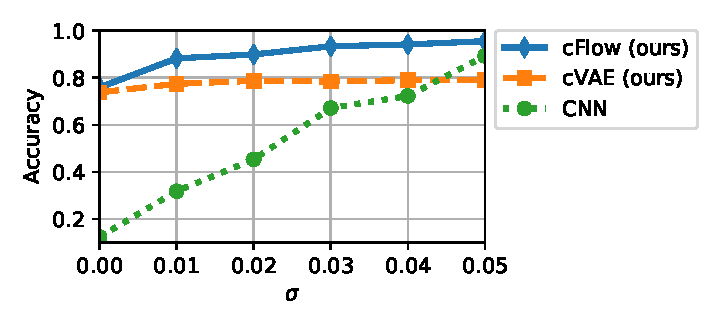
\includegraphics[width=0.6\textwidth]{paper2/Figures/nosinn_cmnist_transfer.pdf}
%   \caption{
%      Results for transfer learning experiments on cMNIST.
%   }%
%   \label{fig:cmnist-transfer}
% \end{figure}

\begin{figure*}[htb]
  \centering
  \subfloat[Performance on cMNIST test data after pre-training on the mixed NIST dataset.]{
      \scalebox{0.6}{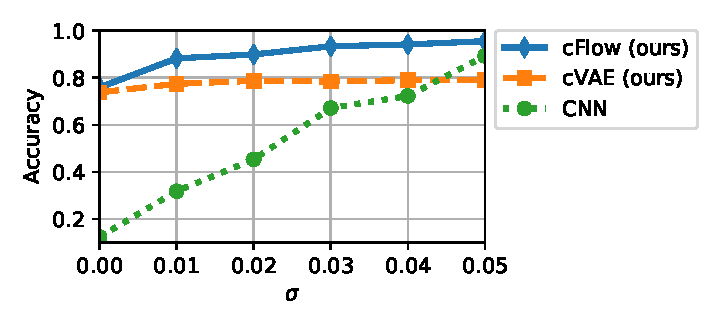
\includegraphics[width=\textwidth]{paper2/Figures/nosinn_cmnist_transfer.pdf}} \label{fig:cmnist-transfer}
  }
  %---
  \vspace{10pt}
 
  \subfloat[Test data input to the cFlow model.]{%
      \scalebox{0.3}{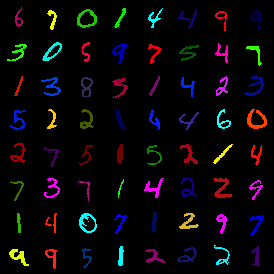
\includegraphics[width=\textwidth]{paper2/Images/cmnist/cflow_tl_original.png}}%
      \label{fig:cflow_tl_original}
  }
  ~~~
%   \hfill
  \subfloat[$\bm{x}_u$ null-samples generated by the cFlow model.]{%
      \scalebox{0.3}{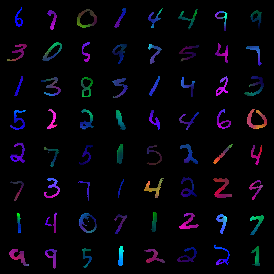
\includegraphics[width=\textwidth]{paper2/Images/cmnist/cflow_tl_xd.png}}%
      \label{fig:cflow_tl_xd}
  }
  
    \subfloat[Test data input to the cVAE model.]{%
      \scalebox{0.3}{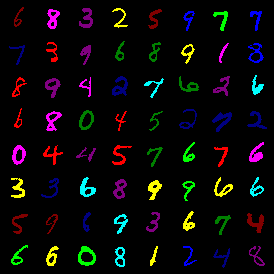
\includegraphics[width=\textwidth]{paper2/Images/cmnist/cvae_tl_original.png}}%
      \label{fig:cvae_tl_original}
  }
  ~~~
%   \hfill
  \subfloat[$\bm{x}_u$ null-samples generated by the cVAE model.]{%
      \scalebox{0.3}{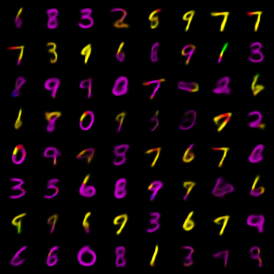
\includegraphics[width=\textwidth]{paper2/Images/cmnist/cvae_tl_xd.png}}%
      \label{fig:cvae_tl_xd}
  }
  \caption{
    Results for the transfer learning experiments in which the representative set consists of colourised samples from EMNIST, KMNIST, and FashionMNIST, while the downstream dataset remains as cMNIST. (a) Quantitative results for different $\sigma$-values. (b-c) Qualitative results for the cFlow model.
    (d-e) Qualitative results for the cVAE model. The qualitative results provide comparisons of the images before (left) and after (right) null-sampling. Note that for some of the cVAE samples, the clarity of the digits has clearly changed due to null-sampling, serving as an explanation for the non-increasing downstream performance.
  }%
  \label{fig:cmnist-transfer-all}
  
\end{figure*}

% \clearpage

% \bibliographystyle{splncs04}
% \bibliography{references.bib}

% \end{appendix}

% \end{document}
